\chapter{Экспериментальный раздел}
\label{cha:research}

\section{Примеры работы}
На рисунке \ref{fig:4.1} приведен пример работы программы.

\begin{figure}[h]
    \centering
    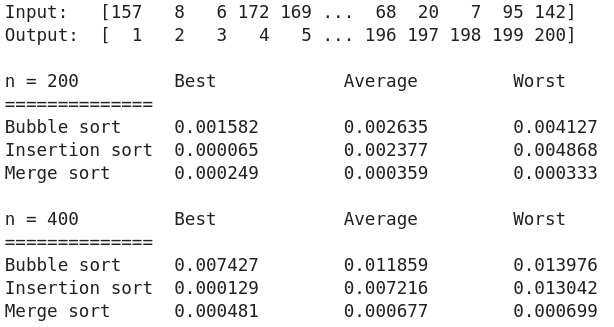
\includegraphics[width=0.6\textwidth]{3/inc/e1.png}
    \caption{Примеры работы алгоритмов сортировки}
    \label{fig:4.1}
\end{figure}


\section{Результаты тестирования}

На рисунке \ref{fig:4.2} приведен результат теста с использованием
фреймворка модульного тестирования в Python: unittest

\begin{figure}[h]
    \centering
    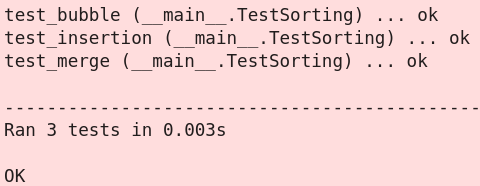
\includegraphics[width=0.5\textwidth]{3/inc/test.png}
    \caption{Результаты тестирования}
    \label{fig:4.2}
\end{figure}


\section{Постановка эксперимента по замеру времени}

Операционная система - Ubuntu 20.04.1 LTS

Процессор - Intel® CoreTM i5-7300HQ CPU @ 2.50GHz × 4

\pagebreak
\subsection*{Сортировкa пузырьком}
\begin{figure}[h!]
    \centering
    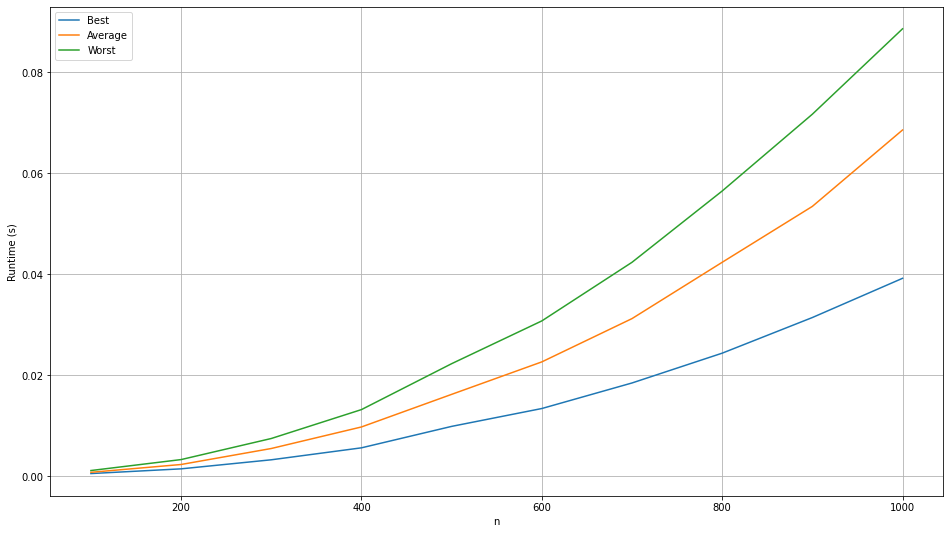
\includegraphics[width=1\textwidth]{3/inc/p1.png}
    \caption{Времени сортировки пузырьком}
\end{figure}

\subsection*{Сортировкa вставками}
\begin{figure}[h!]
    \centering
    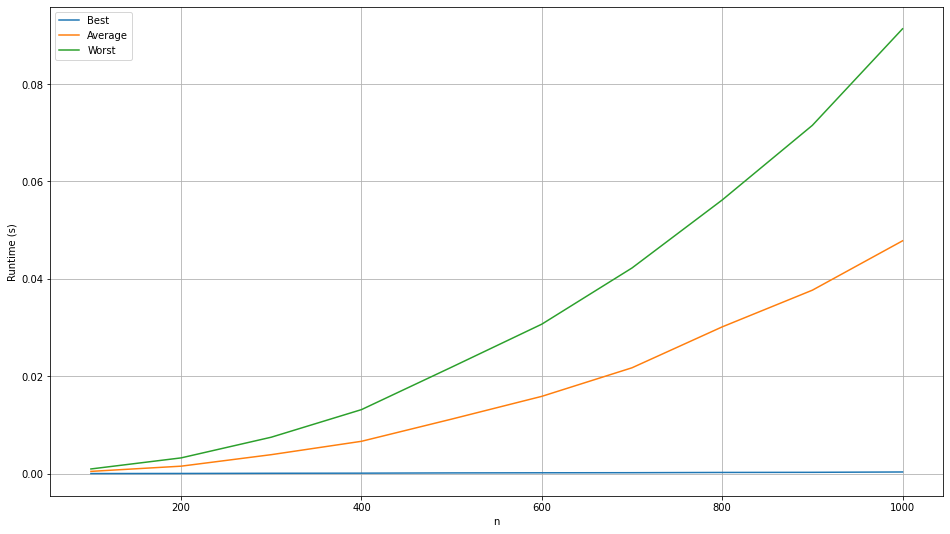
\includegraphics[width=1\textwidth]{3/inc/p2.png}
    \caption{Времени сортировки вставками}
\end{figure}

\subsection*{Сортировкa слиянием}
\begin{figure}[h!]
    \centering
    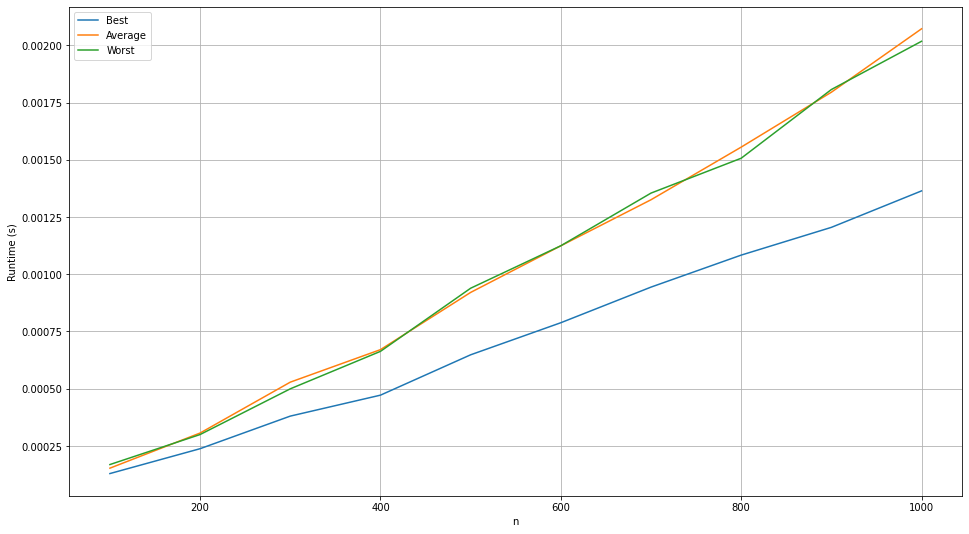
\includegraphics[width=1\textwidth]{3/inc/p3.png}
    \caption{Времени сортировки слиянием}
\end{figure}


\subsection*{Лучшее время}
\begin{figure}[h!]
    \centering
    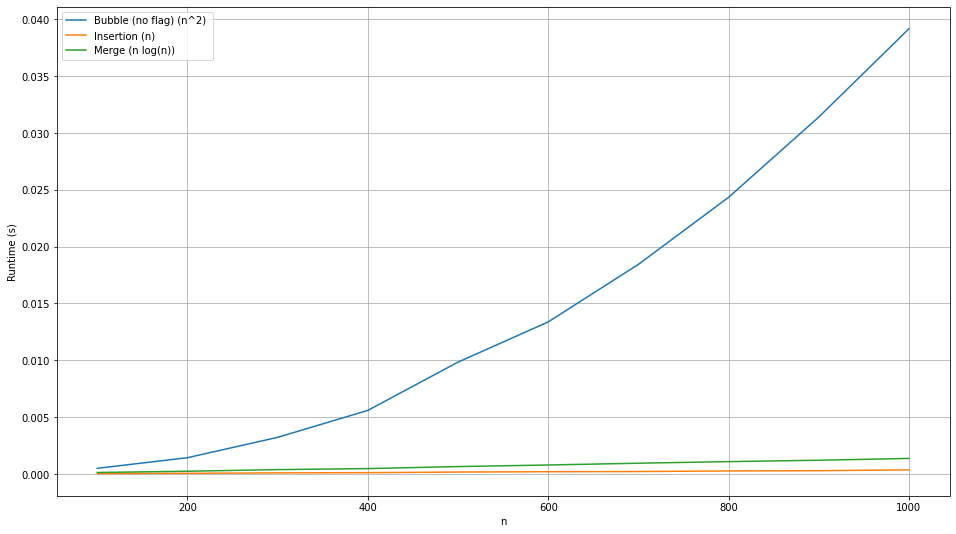
\includegraphics[width=1\textwidth]{3/inc/p5.png}
    \caption{Сравнение лучшее времени работы алгоритмов}
\end{figure}

\clearpage
\subsection*{Среднее время}

\begin{table}[h]
    \centering
    \csvautotabular{3/inc/average.csv}
    \caption{\label{tabular:benchmark} Среднее времени работы (ns)}
\end{table}

\begin{figure}[h!]
    \centering
    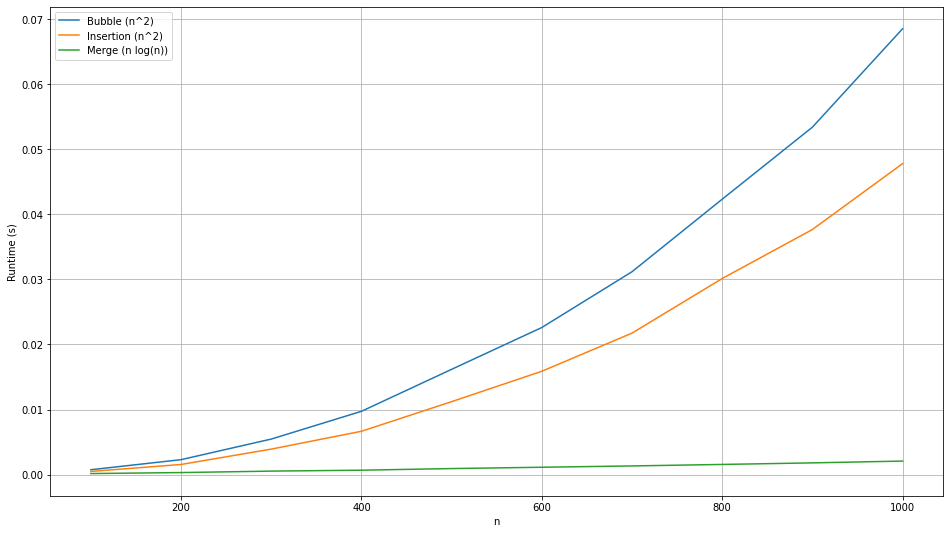
\includegraphics[width=0.95\textwidth]{3/inc/p4.png}
    \caption{Сравнение среднее времени работы алгоритмов}
\end{figure}



\section{Вывод}

Из графика мы видим, что алгоритм сортировки слиянием работает со сложностью
O(nlog(n)) во всех случаях и является наиболее оптимальным,
алгоритм сортировки вставками является лучшим, если массив уже отсортирован или почти отсортирован.
Сортировка пузырьком используется в основном как обучающий инструмент.
На массив длины 1000, сортировка слиянием в 30 раз быстрее сортировки
пузырьком и в 23 раз быстрее сортировки вставками по сравнению среднее времени работы.
